\documentclass[a4paper,12pt]{report}
\usepackage[utf8x]{inputenc}
\usepackage{graphicx}
\usepackage[normalmargins,normalleading]{savetrees}
\usepackage{listings}
% Title Page
\title{Developing a Hand Gesture Interface to Issue Commands to an Autonomous Quadrocopter}
\author{Jeremy Hurst}


\begin{document}
\maketitle

\begin{abstract}
As the complexity of robotic functionality increases and robots become more useful in everyday life, robotic control will have to become more user friendly while maintaining the ability to issue high level commands. One of the most natural ways humans communicate and issue commands to each other is by making gestures. This paper explores the challenges involved and the steps that need to be taken in order to create a hand gesture interface for robotic control. This knowledge is then applied to an implementation of using hand gestures to control a flying quadrocopter.


\end{abstract}
\tableofcontents
\newpage
\maketitle

\section{Methods for Hand Gesture Recognition}

\subsection{Introduction}

A hand gesture interface could provide an attractive alternative to current human computer interfaces which are cumbersome. Hand gestures are easy to learn and memorize, can be performed with speed and ease, and are complex enough to  allow a large vocabulary of gestures which are distinguishable due to their diversity.  Currently we use mouse and keyboard almost exclusively to issue commands to our computers. Keyboards and mice may be sufficient as control interfaces for many tasks, but for some they are suboptimal. Most popular computer applications used today have countless different functions which are accessed by traversing the mouse pointer through a maze of drop down menus, these functions could be much more easily accessed by using a hand gesture interface. Robotic control would also be improved by a hand gesture interface where any sort of control hardware would become inconvenient to use.   
Gestures are a very powerful means of communication, so powerful in fact that our entire language can be translated into hand gestures and used as an efficient way of communication for disabled persons (Sign Language). Consequently a significant amount of research has gone into making human-computer interfaces which can recognize hand signals \cite{1} \cite{2}. Many appearances of hand gesture recognizing human-computer interfaces in science fiction have demonstrated the excitement people have for and the possibilities of such an interface. 

The mechanical devices we use today for interaction with our computers are good for some tasks, but cumbersome for others. Three dimensional computer automated design, for instance, could greatly be improved because the devices we use today such as mice and most joysticks can give accurate input in two dimensions, but they are manipulating virtual objects in three dimensions. All of the implementations of three dimensional manipulation with a two dimensional input are non intuitive and awkward. Effectively the user is trying to manipulate a three dimensional object while being constrained to move in two dimensions. If three dimensional gesture recognition were applied to 3D CAD, computer design software could be as intuitive to use as molding clay. 

The following is an evaluation of a number of techniques that have been used to create human gesture interfaces for computers using the hardware and software which we have today. 

\subsection{Challenges Involved}

A number of requirements for an effective hand gesture recognition interface make the problem particularly challenging \cite{egm}. A good hand gesture recognition interface must 1) be person-independent. The interface should recognize the same hand gestures from hands of different color and size. The interface must 2) be able to distinguish the hand from the background of the picture, no matter how complex. All of these are problems which can require computational algorithms which are complex and computationally expensive. All of these algorithms which have been developed with an open source license have been organized into libraries called OpenCV. OpenCV makes hand segmentation and gesture recognition less difficult and makes coding less cumbersome. 

\subsection{Gesture Recognition Using a Full Color Webcam with 240 X 380 pixel resolution and OpenCV libraries}

This approach takes advantage of the open source library for image processing called OpenCV \cite{opencv}. In this approach, hand gesture recognition is taken in three steps: hand segmentation based on characteristic color values of the human skin, hand tracking, and gesture recognition. The hand segmentation in this case is computationally simple because all that needs to be done is to subtract everything from the image which is not the color of the skin on the human hand. Gesture recognition is done by extracting several hand features that are fed into a finite state classifier which identifies the hand configuration.  In order to make gesture recognition for this approach more accurate, tracking needs to be implemented. Tracking is performed by assuming that the hand retains constant velocity and using a pixel labeling approach which keeps track of individual features of the had as it moves from frame to frame. 

This method boasted a 98 percent correct interpretation rate among 40 different people doing 40 distinct hand gestures in different lighting conditions and backgrounds. It was then applied to being used as a controller for a 3D video game and was effectively used for movement commands for the game

\begin{figure}[H]
\centering
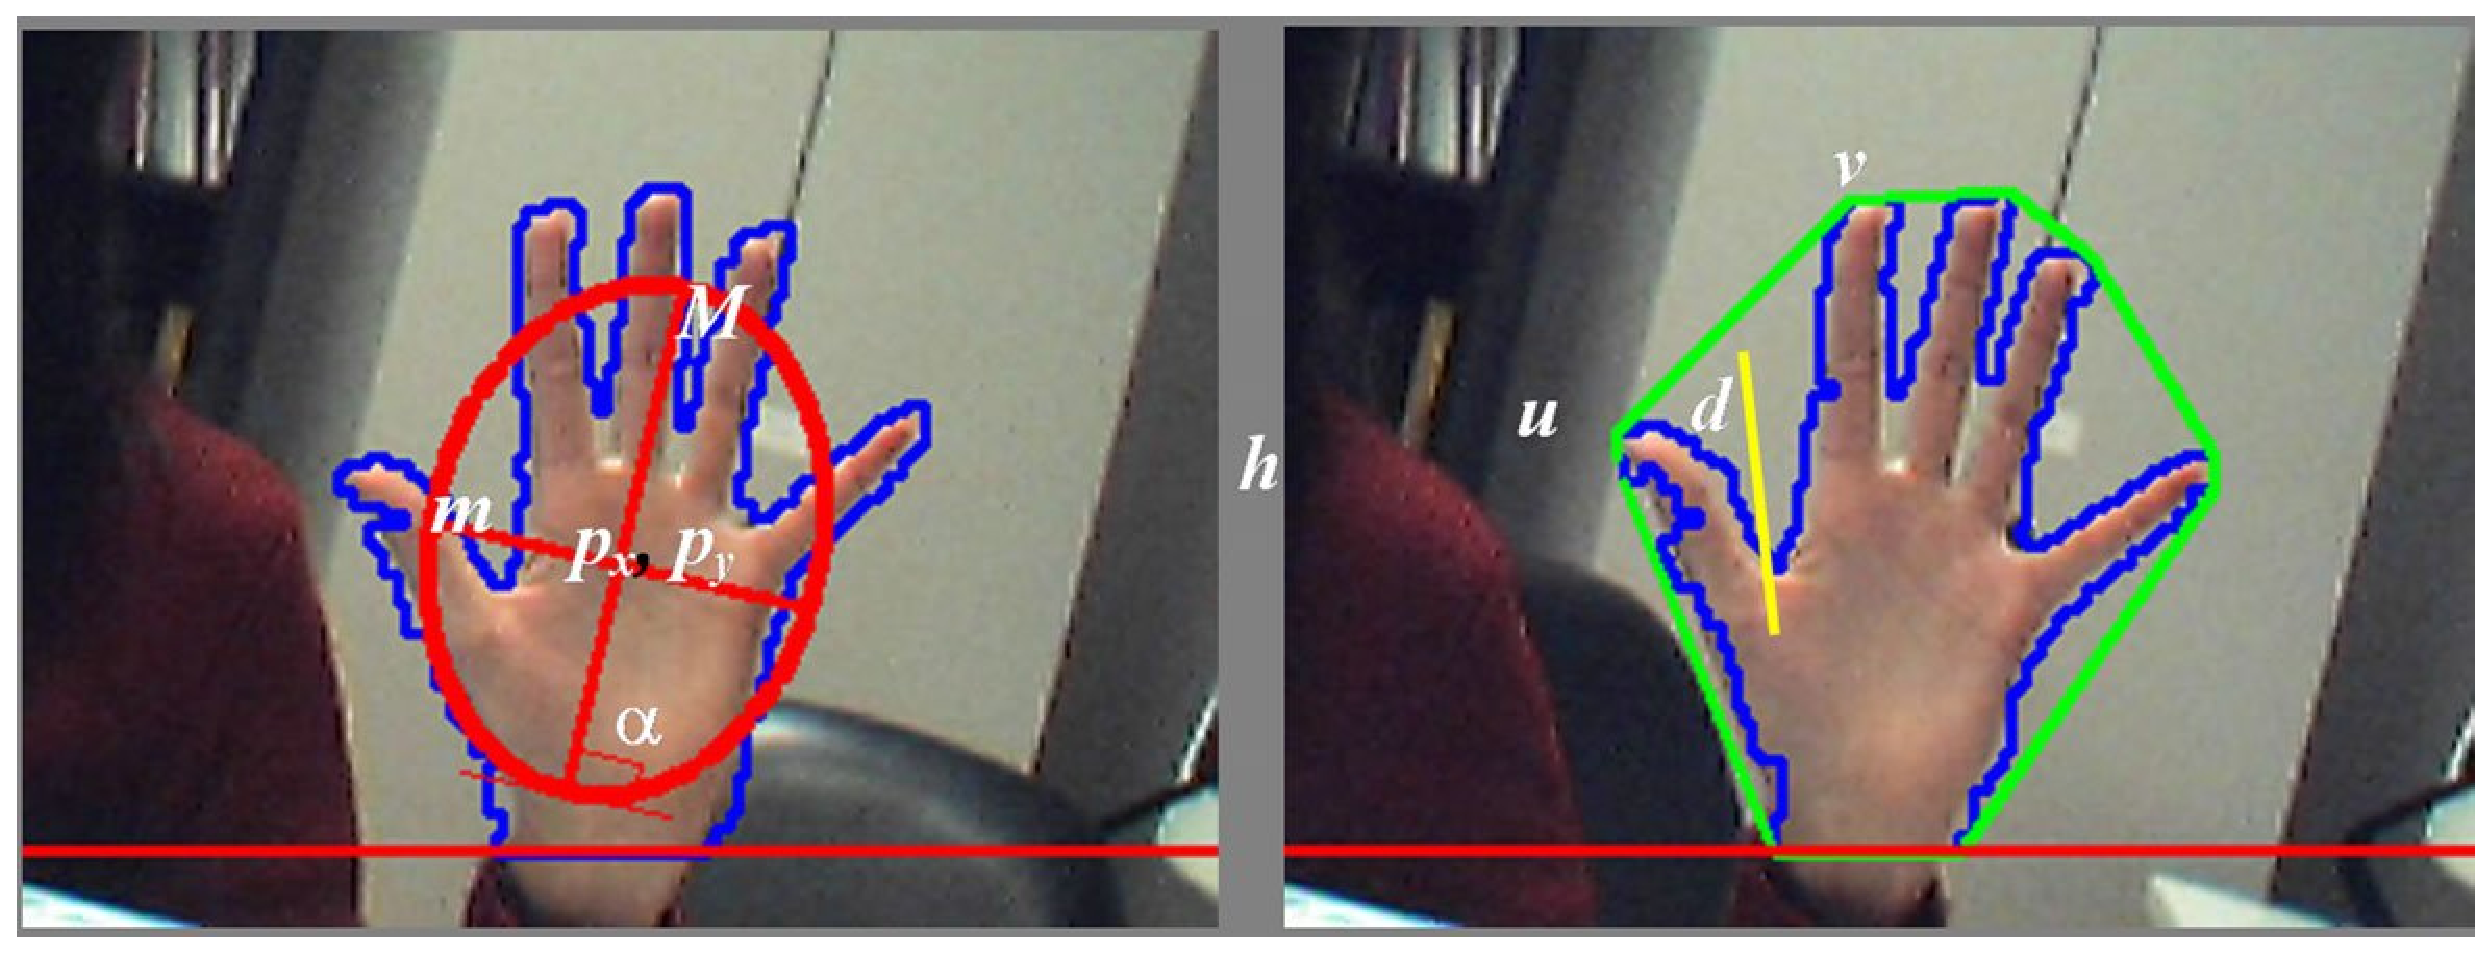
\includegraphics[height=60mm] {opencv.eps}
\caption{An application of OpenCV libraries for use in hand segmentation and hand posture recognition}
\end{figure}



\subsection{Finger Tip Tracking using Color Markers}

A popular method for hand signal recognition using a color sensitive webcam is to have the user wear markers on the tips of their fingers which all have a unique color \cite{sixthsense}. The markers can be easily identified in the program by searching for a group of adjacent pixels which have the distinct color of one of the markers. Once the fingertips are identified, their position is stored as individual points. All that is required to do gesture recognition is to an analysis based on the positioning of those points in relation to the other points. This process makes both segmentation from the background and interpretation of the hand gesture computationally simple and is an attractive method for people who want to do person independent hand gesture recognition with inexpensive hardware. The producer of this device called SixthSense claims that he will release all of his software open source, a search for the code has yielded no results.

\begin{figure}[H]
\centering
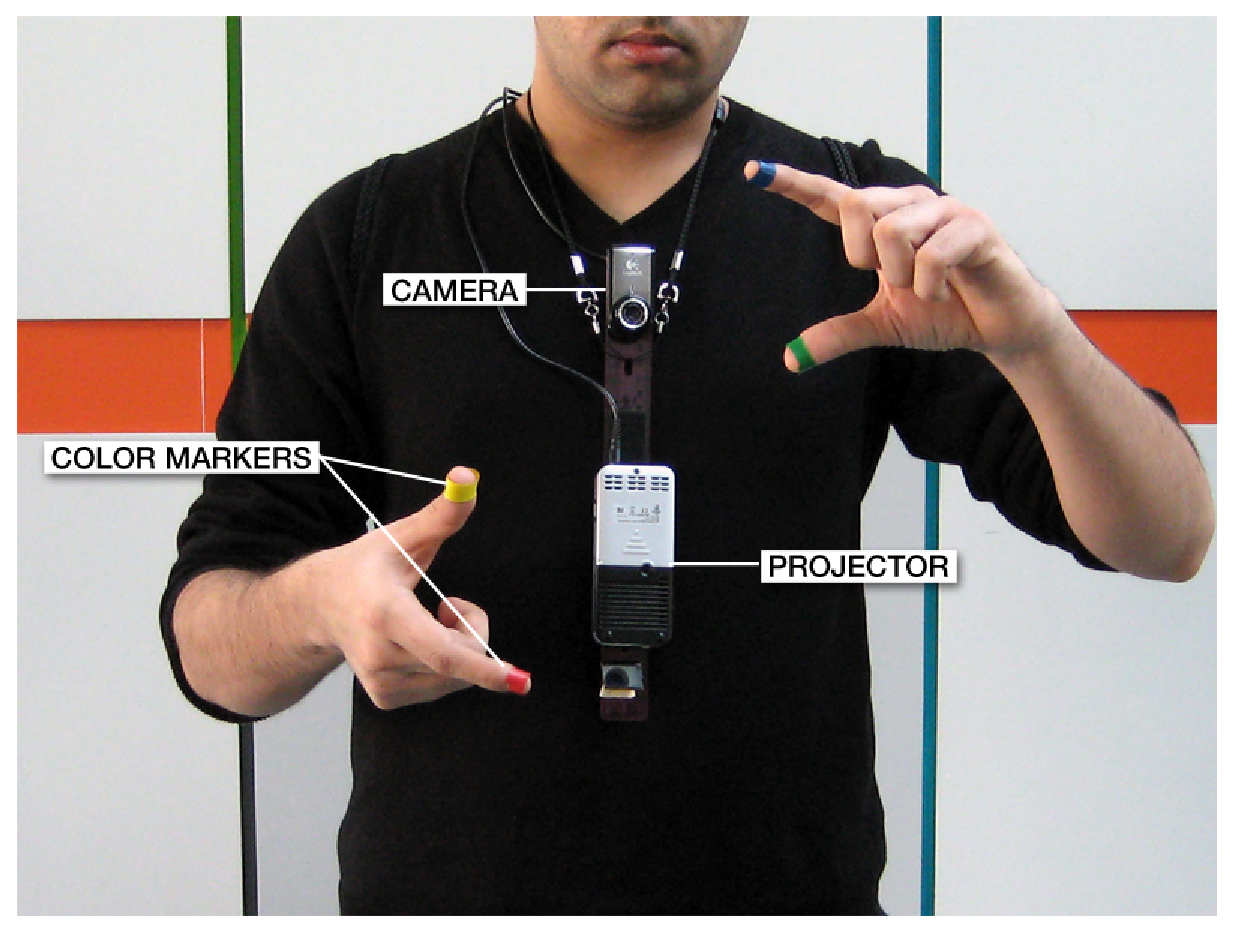
\includegraphics{sixthsense02.eps}
\caption{Using distinct color markers on the tips of fingers to track the position of index fingers and thumbs. This device would project the image of the environment the user was manipulating right infront of him/her. The objective was to create a more mechanical way of interacting with portable computers}
\end{figure}


\subsection{Finger Tip Tracking without Color Markers}

A group of researchers from University of Tokyo\cite{fingertip} have come up with a novel idea for gesture recognition for use in a computer interface. The process they use has two main steps. First they extract the hand from the rest of the picture, then they run an algorithm which scans through the image of the extracted hand to find the features of the hand which can be identified as fingertips. 

They recognized that it is a very complex problem to extract the hand from a non uniform background. In order to solve this problem, they used an infrared camera which was calibrated to be sensitive to the wavelength which our body heat naturally emits (between 30 and 34 degrees Celsius)  The resulting picture was one which had a uniform background shade and a uniformly intense shape of the hand. Extraction of the hand from the background in this case is computationally simple because all that is required is a threshold value be chosen and all of the pixels in the image that are darker than that value get set to black and all of the pixels which are brighter get set to white.  

In order to find the tips of the fingers on the newly extracted image, they first define searching windows whose size is proportional to the width of the wrist in the image, then they have the computer iterate through the image with that scanning window. The scanning window is large enough so that it can fit enough of a fingertip inside to properly identify it as a fingertip, but not big enough to contain two different fingertips. As the scanning window scans through the image, when a fingertip is identified, it's position is saved and after the scan is complete, all of the positions of all of the fingertips that were identified are saved in memory. At this point the hand gesture can be interpreted by doing a geometric analysis (similar to the one in the previous section) on the fingertip positions. This method would not be useful in cases where the background of the infrared image was not cooler than body temperature. It would not work well, for instance, if a user had other parts of their body in the picture. For the purpose of a top-down view of the desktop environment, however, it works just fine.

\begin{figure}
 \centering
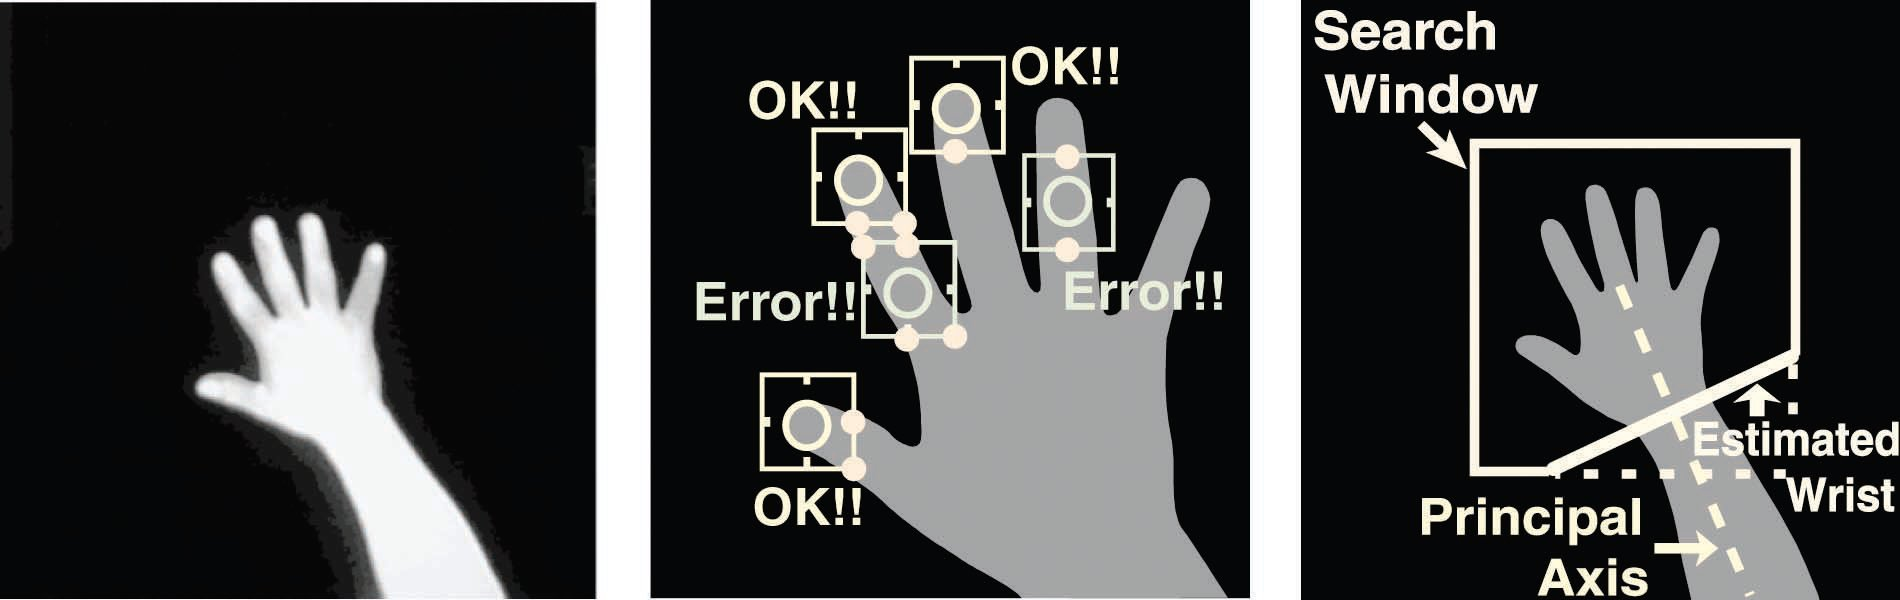
\includegraphics[height=50mm] {fingertipinfored.eps}
\caption{The top-down infrared image of a human hand and the a visualization showing how fingertip detection was implemented}
\end{figure}


\subsection{Elastic Graph Matching}

Elastic Graph Matching (EGM) \cite{egm} is an image recognition architecture which was inspired by a neural information processing concept called the Dynamic Link Architecture\cite{dla}. EGM has the advantage over other techniques for hand gesture recognition in that it does not require a previously segmented input image. In EGM, images are represented as two dimensional labeled graphs, the nodes of the graphs are labeled with a local image description, and the edges of the graph are labeled with a distance vector. Elastic matching on the produced data involves searching for node positions such that the local image description attached to each node matches the image region around the node and that the graph is not distorted too much\cite{egm}. The result of past implementations of this process have taken 58 seconds per image on a workstation which was running a single core 200mhz processor which had 340MB RAM and it was able to recognize 28 different hand gestures in front of complex backgrounds with a 93.1 success rate.

\begin{figure}
\centering
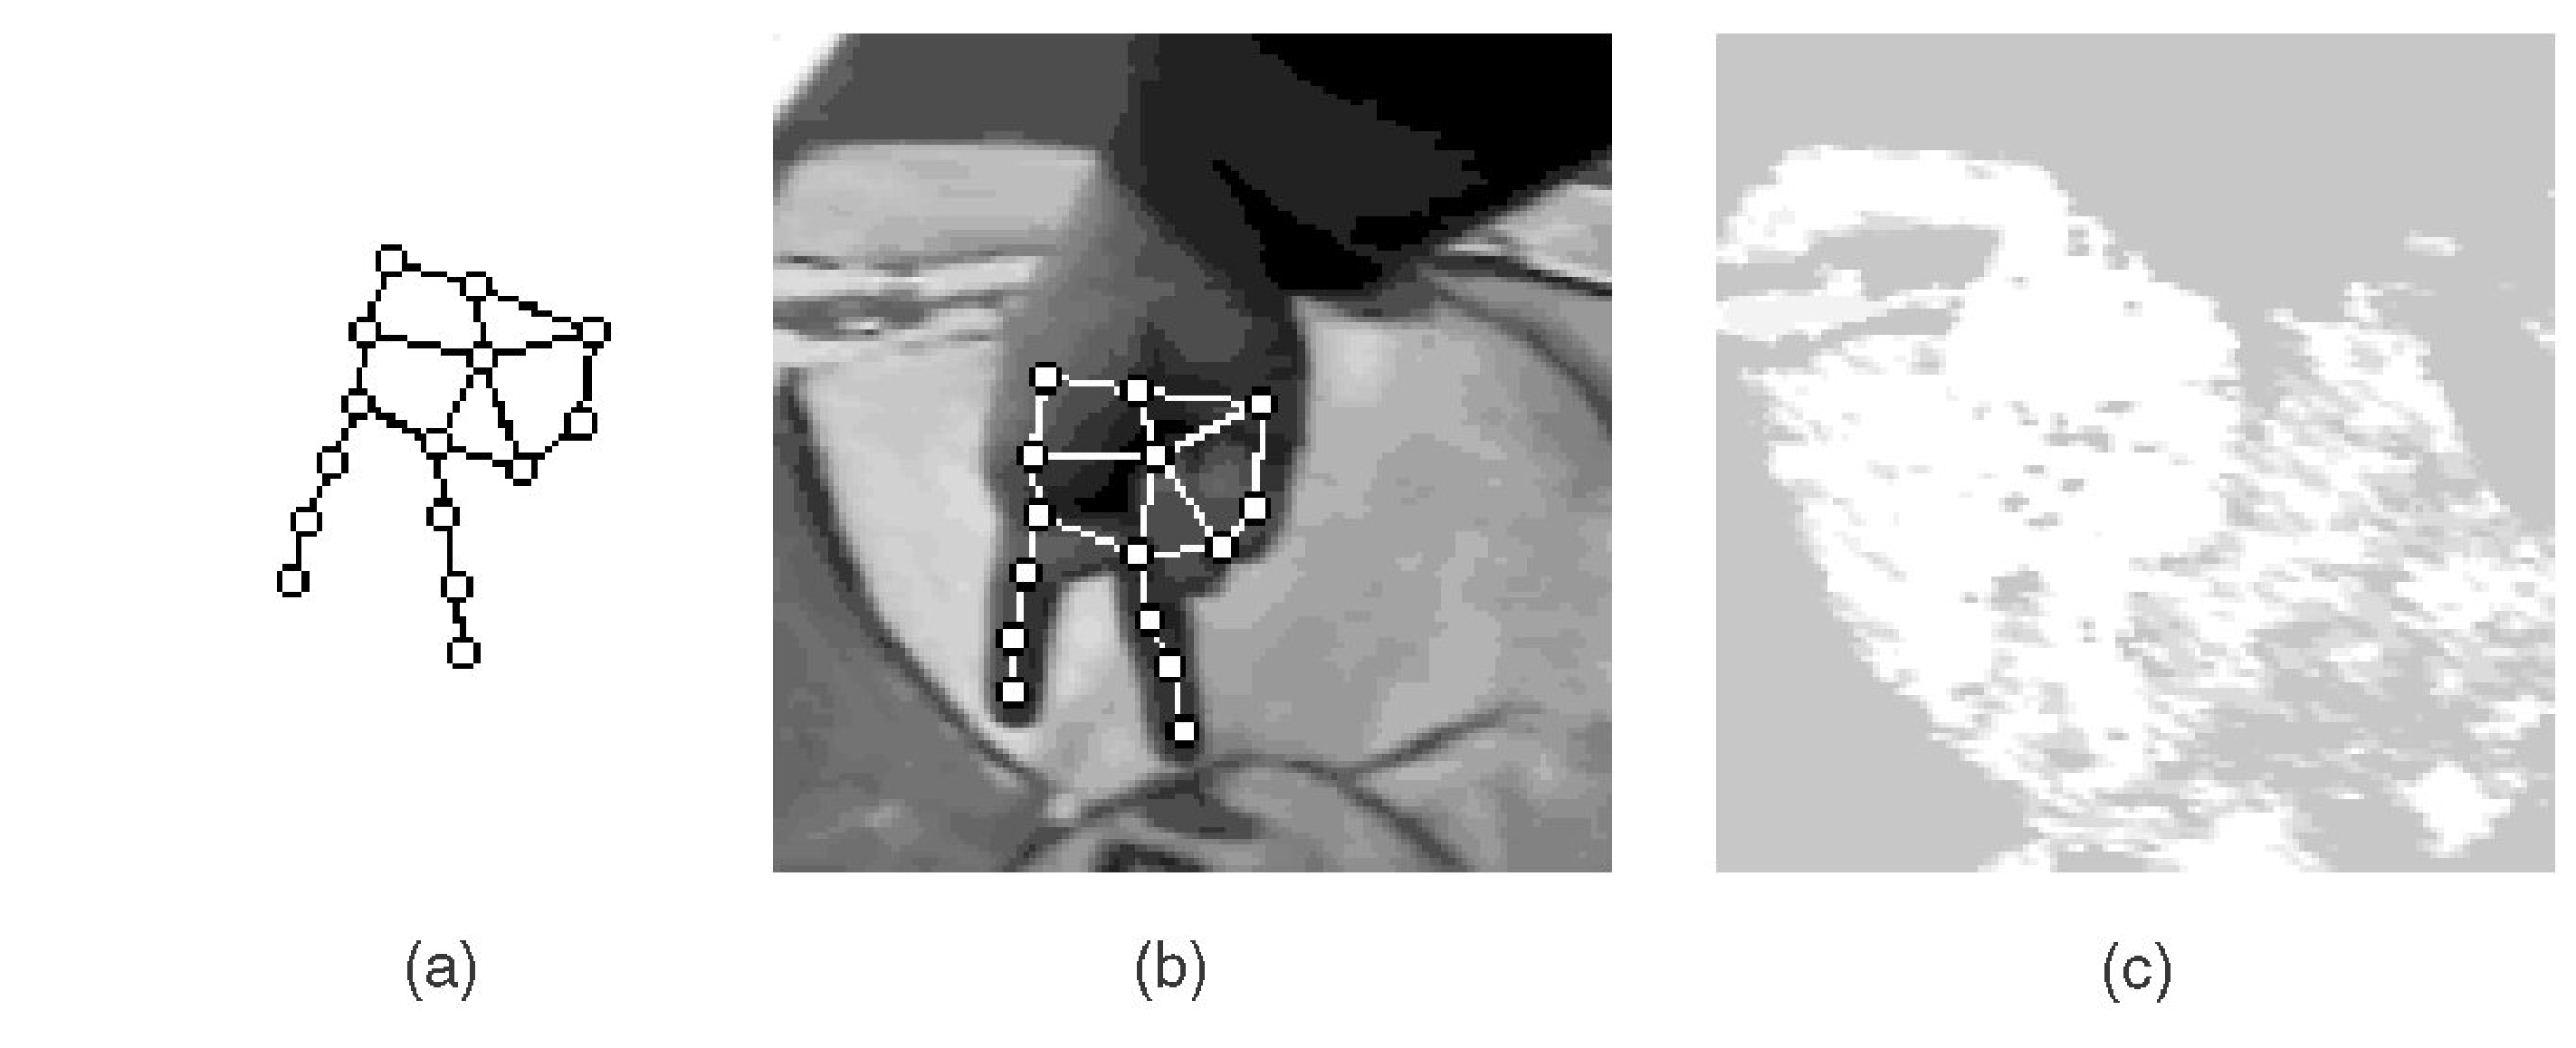
\includegraphics[height = 60mm]{egm.eps}
\caption{Two dimensional elastic graph matching for hand posture recognition}
\end{figure}



\subsection{3D Hand Posture Estimation using Training Contour Variation}

This technique uses a computer model of a three dimensional hand and matches the two dimensional profile of the user's hand to the three dimensional model \cite{3d}. The first part of this technique involves extracting a profile of the hand from the two dimensional image such that the only thing left after the extraction is a black background with a white outline of the hand. The variations of possible shape appearances of the hand outline are trained to images generated by the computer based on perspectives of the 3D model of the hand. The possible variations are then represented as the "Locally-Compressed Feature Manifold (LCFM) in appearance feature space." \cite{3} \cite{4} The posture tracking is done by tracking posture of the virtual hand created by the computer and represented in the LCFM. 

This process is a good way to determine exactly what position the hand is in. Implementation of this method have resulted in correctly interpreting the hand posture 99.1 percent of the time \cite{3d}, but it is also extremely expensive in computational terms. If someone wanted to use this as a human computer interface, they would have to add to this a library of hand gestures and a feature which would compare the posture of the hand to determine if the current hand position is a gesture. 

\begin{figure}
\centering
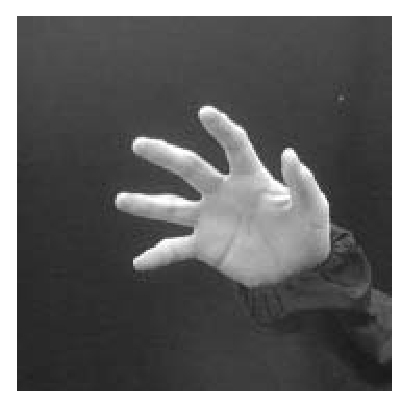
\includegraphics[height=50mm]{3d1.eps}
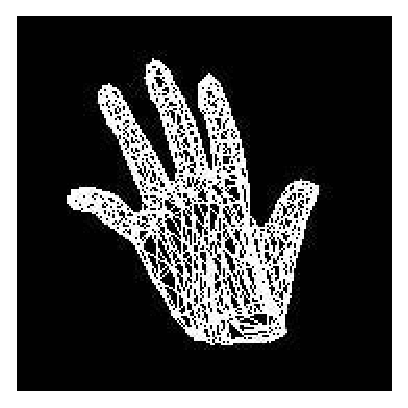
\includegraphics[height=50mm]{3d2.eps}
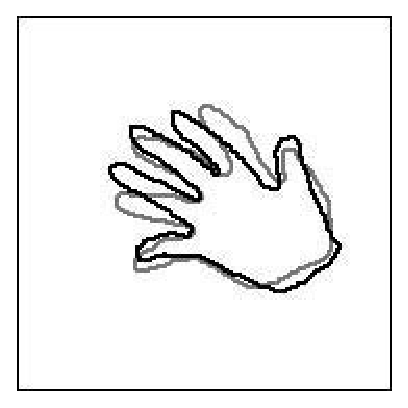
\includegraphics[height=50mm]{3d3.eps}
\caption{3D hand posture estimation using training contour variation. First, the initial image (top left) is processed and returned as a 3d node graph (top right) and then simplified to a two dimensional outline (bottom center)}
\end{figure}



\subsection{Evaluation}
Nearly all of these methods for hand gesture recognition involve two parts: hand segmentation and gesture interpretation.  Some forms of hand segmentation may be better for certain situations and not so good for others. In the same way some forms of gesture interpretation may be better for some situations than others. When working on this problem, the right combination of hand segmentation and gesture interpretation should be used.   

\section{This Project}
For this project, I used a software module called colormap to do the segmentation and I programed the gesture recognition myself. 
\subsection{Overview}
In 2010, Parrot, a company which specializes in wireless devices, released a product called the AR Drone which is a quadrocopter with a multitude of onboard sensors with the intended use of being controlled by iPhone and iPod touch for "Augmented Reality video games". When they released the product, they also released the control software with an open source license. 

This has had a huge impact on the world of research in robotic control. When using other robots for research projects. A major component of any project involving robotics is interfacing the hardware such that it can be controlled by computers. The complexity of the AR Drone with all of it's sensors and four different propellers which need precise individual control would have made it very difficult to program alone.  

Since the software that has been developed by Parrot has been released open source, students who want to do research with the AR Drone do not have to worry about all of the difficulties of hardware interfacing. They can just run the advanced control functions that Parrot developed to control the quadrocopter. These control functions have been added to the open source library for robotic control and the new language known as URBI. With the use of Gostai Labs, I was able to upload urbiscript that I had written to the AR Drone and view output from the drone in the form of its camera feed, echo commands from within the urbiscript, and floats which were being modified while the drone was operational.

\subsection{Hardware}
The AR Drone Specifications:
\begin{itemize}
 \item Onboard Computer:
CPU: ARM9 468MHZ embedded microcontroller
RAM: 128 MB
\item Operating system: Linux with Busybox
\item Sensors:
Cameras: Front: wide-angle (93 degrees) resolution: 640X480 Frames Per Second: 30, Bottom: 64 degrees, resolution: unknown, Frames Per Second: 60
Ultrasound Altimeter: Capable of detecting the ground up to 12 meters away
\item 3-Axis gyrometers and accelerometers for three dimensional position feedback 
\end{itemize}
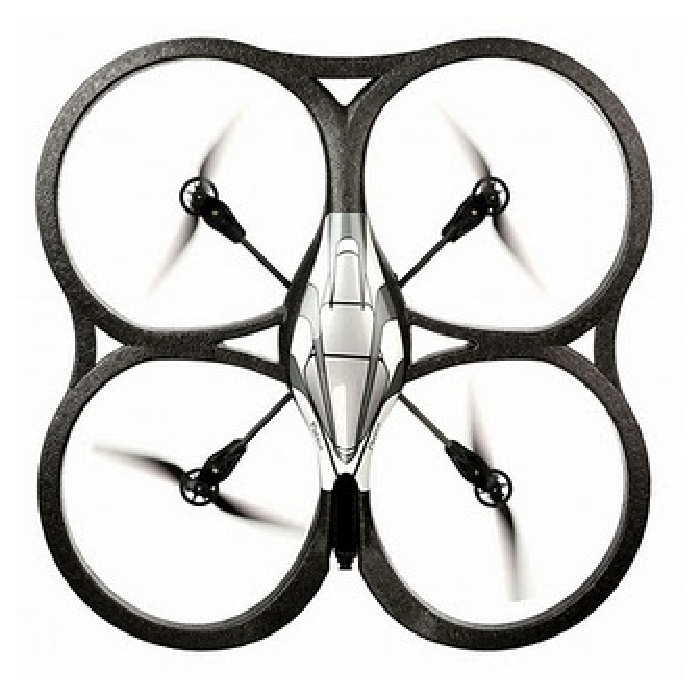
\includegraphics{top_down.eps}
	
\subsection{URBI and URBI Modules}
The growing diversity and complexity of existing robotic devices like humanoids 
or wheeled robots, has lead to the development of several incompatible software interfaces to control these robots. 
URBI which stands for a Universal Robotic Body Interface is an attempt to make a standard language for robotic control of complex systems.URBI is a scripting language which is syntactically similar to C and C++ with some influences from Python. In this project I used URBI to program the AR Drone

Participants of the open source community have added to URBI by creating modules which you can use for specific purposes. URBI modules are similar to C++ header files and they add some functionality to the URBI language. In this project I used the colormap URBI module to detect objects with a certain color signature and return their position on the screen.
\subsection{Software}

Gostai Lab is commercial software which is a powerful tool one can use to graphically design a GUI using parameterizable widgets that can be simply dragged and dropped on a customizable layout.You can then export your interface as an application to remote control a robot, monitor sensors, cameras, or use the console to directly send urbiscript commands to your robot. I used Gostai Lab in this project so that I could view outputs from the AR Drone such as live video feed from the Drone's camera, what the colormap module detects in the feed, and the x and y coordinates of the object colormap detects. I also used Gostai Lab to upload my urbiscript files to the AR Drone.
\subsection{Final Result}
The full capabilities of the drone at the end of my project included being able to have the drone takeoff, land, spin right at varying speeds, spin left at varying speeds, and return the x and y coordinates of the object colormap was tracking in the range of -.45 to .45. My goal was to have a robot which would recognize multiple gestures and behave in distinct ways with respect to the gesture it recognized. I decided that the most robust way I could do gesture recognition would be to store the positions of the object with respect to time and interpret the gesture based off of the information stored.In terms of how to make a recognizable change in behavior of the drone, the best way to do this seemed to be outputting the result of the gesture interpretation in binary. Since the quadrocopter could spin left and right, I assigned left to being 0 and right to being 1. This would allow for a maximum of possible visual outputs for the number of hand gesture inputs.

What I ended up doing was defining four different regions of the image returned by the AR Drone as numbers one through four. After the AR Drone was initialized and it was ready to record the gesture, if the object traveled into any of the regions previously mentioned, it would record the value of that region. After it had stored four values, it would take the sum of those values and output the result in binary as left and right spinning motions of the AR Drone in a sort of dance. 

\begin{figure}
 \centering
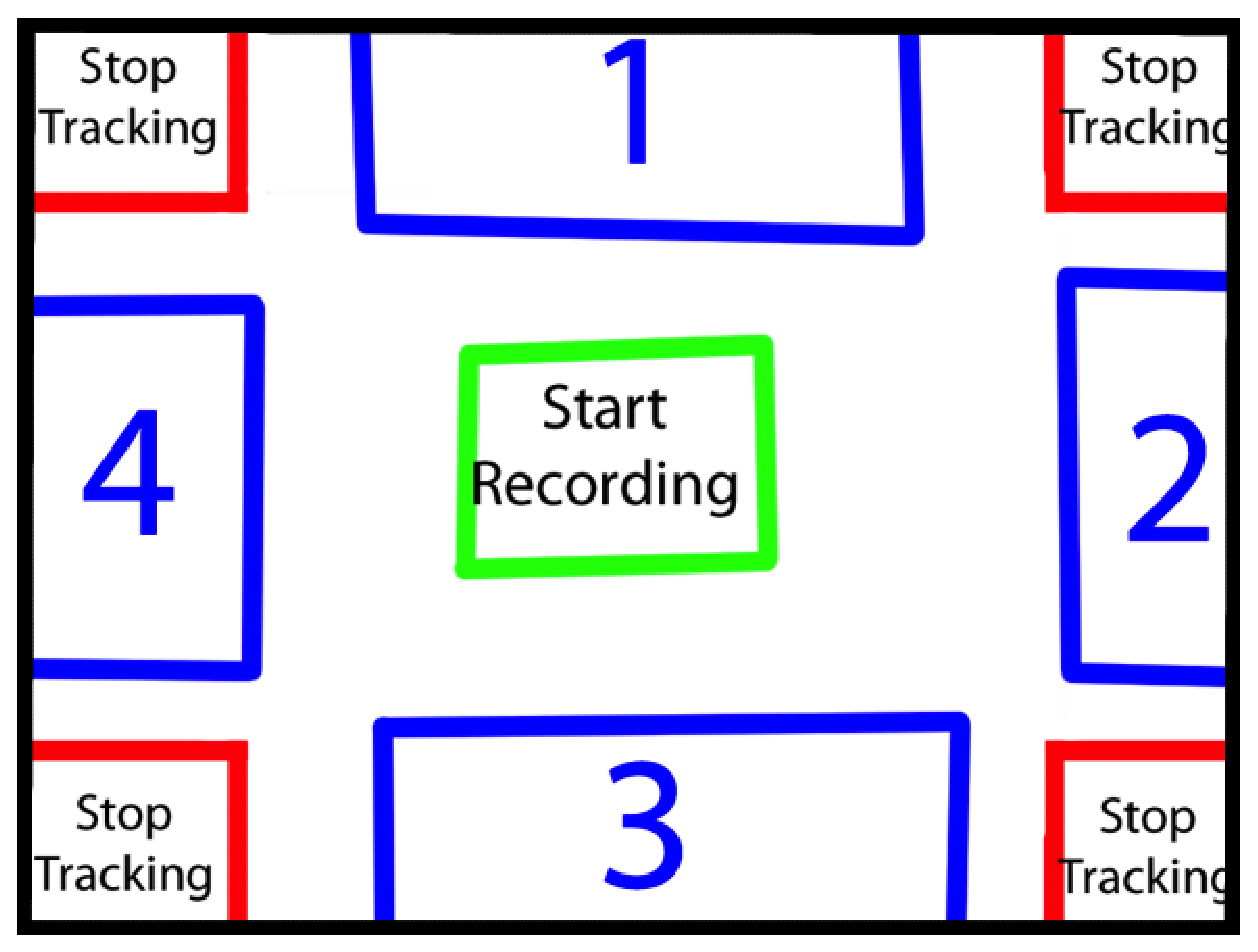
\includegraphics[height=100mm] {image_sections.eps}
\caption{The sections of the drone's camera view which had particular functionality. The regions with numbers would save that number in memory when the object moves into that region}
\end{figure}

When the urbiscript was first initialized on the AR Drone and after the drone had taken off, the drone would be initialized in the balltracking state and would continue tracking the red color source until the source was in the 
corner of the returned image (x * y $>$= 0.09). When the drone would stop tracking, it would be ready to start recording the hand gesture, but would not actually begin recording until the color source was put into the center of the drone's vision. Having tracking stop when the color source was in the corner of the returned image was a great way to give visual feedback to the user that tracking had stopped and the drone was ready to record because in order to get the color source into the corner of the image while the drone was tracking the color source, they would have to move the color source into a region of the returned image which would make the drone spin at it's maximum speed. The result was a contrast between spinning at its maximum speed and completely stopped which could easily be recognized by the user. The reason I had recording start once the color source was in the center of the image was that I needed the gesture to always start from the same state where none of the regions which are recognized as part of the gesture would be tripped during the initialization of the recording stage.

Once the color source moves to the center of the returned image and tracking is off, the drone would then record four numbers, none of which are the same as the number previously recorded. Whenever the color source moved into one of the four regions which are declared as gesture recognition regions the number for that region would be recorded as long as the previous number was not the same as the number for the region the color source was currently in. This was to prevent all of the memory being filled up with one value because it would recognize that the color source was in a gesture recognition region for four tenths of a second (the time it would take to fill up four memory values for every 0.1 seconds the recognition loop executes). 
Once the four memory slots are filled with the region numbers, the program exits the recognition loop and proceeds to the next section of the program which takes the sum of those numbers and then outputs the result in the binary dance where spin right is 0 and spin left is 1.

I considered setting the color threshold settings in colormap to instead of track the color red to track the RGB color of my hand. This would enable me to track the x and y coordinates of my hand as opposed to the ball that I hold. This would mean that I could do hand gestures with only my hand and I would not need to hold a red ball and it would make hand gestures more natural. The problem I found with it was that the skin color of my face was within the color threshold of my hand which meant that my hand gestures would be interfered with if my face was in the image. It also meant that the AR drone would track my face and recognize gestures when I moved my face around.  

\subsection{Programming in Urbiscript}

A limitation that I found in working with urbiscript is that within a myTag loop, there cannot be multiple if statements. In order to have the same functionality, I needed to translate multiple if statements into a chain of if else statements. For instance the following code would not be syntactically correct in urbiscript:

\begin{lstlisting}
myTag: (every 0.1s)
{
  if (condition == 0)
  {
    do this;
  }
  if (condition == 1)
  {
    do that;
  }
};
\end{lstlisting}

Instead you would have to write it like
\begin{lstlisting}
myTag: (every 0.1s)
{
  if (condition == 0)
  {
    do this;
  }
  else
  {
    if (condition ==1)
    {
      do that;
    }
  }
};
\end{lstlisting}

to have the same functionality. 

The structure of my final program was as follows: Initialization, Gesture Recognition, and then Output Implementation. During the initialization phase, all of the different variables (including event switches and gesture memory) would be set to the values appropriate for entering the loop for the first time. During the Gesture recognition phase, the behavior of the drone would change from tracking the ball to recording the gesture based on event switches. In the output implementation stage, the sum of the regions detected would be taken and translated into binary, then fed as instructions to drone movement. 

\begin{figure}
 \includegraphics[height=200mm] {flowchart.eps}
\caption{A flowchart of the urbiscript program I wrote for gesture recognition }
\end{figure}






\section{Possible Future Projects}
If I were to continue working on this project, I would improve the functionality of the AR Drone by changing the following things:
\subsection{Ratio Color Tracking}
  Current methods of object identification and segmentation by color are brittle; they only work correctly with proper lighting conditions. According to current methods, a red ball would only be red with the right amount of lighting. This is because current methods of color detection scan an RGB image with pixel color values in 8 bits meaning values between 0 and 255 for pixels which fit color within a certain range. For instance, if the color segmentation program was to scan through the picture and identify all of the pixels which are red, what it looks for are specific pixels which have color values within a certain range, say red between 240 and 255, 0 green, and 0 blue. 

The reason this method is incorrect for color recognition in the real world is that it scans for pixels with an absolute color, not pixels with relative color. Something is still red when it is dark red, but the scanner would not identify it as red because the red value would not be high enough to register as red. What matters in the real world is not what range of color the pixel fits within, but the relationship between the colors. 

A method to do this would be to form relationships between all three values by division, R/G, R/B, G/R, G/B, B/R, B/G, and then specify the range those relationships can be in order to identify that specific color. For example, consider that an object which we want to track has in full lighting conditions RGB values of (255, 1, 128) sort of a reddish purple. In this case, R/G would be 255, R/B = 2, G/R = 1/255, G/B = 1/128, B/R = .5, B/G = 128. In darker conditions, these ratios should stay within a certain range, but would be relatively similar. I expect that this method would allow balltracking to work in multiple lighting conditions. Perhaps there is a better mathematical model which could be made to best for this task, but a relational model would no doubt be a superior method for segmenting and distinguishing which pixels are of what color.

An application of this to my project would be to program the AR Drone to track an object in multiple lighting conditions. This could be done by modifying the colormap URBI module so that it would behave in a completely different manner as described above.   
\subsection{Moving Object Segmentation}
A way in which I could improve the object detection based on color would be to program colormap to recognize a blob of color which is in motion. For the purpose of gesture recognition, you need to have the computer only pay attention to the blob of the color of interest which is in motion. In the scenario that the color of the object which you want to track is in the image for things other than the object which you want to track, it would be useful to determine which part of the color segmented image is in motion. For instance, people's skin color pretty much stays constant independent of where on the body the skin is. If someone wanted to have the AR Drone track their hand gesture while other parts of their body were in the camera's view, if they were using the colormap URBI module, they would be unable to do it because colormap would return the x and y coordinates of the center of the weighted average of the position of all of the pixels with that color in the image. 

In order to fix this, colormap needs to be able to distinguish the part of the image which would be the hand. A way in which this could be done would be to identify individual blobs of the desired color within the image, track each of their positions with respect to time over multiple images, and determine which blob of that color is moving the most. 

\section{Conclusion}

The purpose of this project was to prove that a hand gesture interface could be applied to a flying quadrocopter to issue a multitude of different commands. With the success of this project, I have proved that gesture recognition is certainly a viable way to control robotics. If ever one is in the situation where they need to control a robot which has a camera and they need to issue it commands without standard input devices, gesture recognition may be a preferred option to other alternatives such as voice recognition. Whereas in voice detection and interpretation, it is extremely difficult to remove the person's voice from background noise, with gesture recognition, you can put a flash on the robot to ensure reliable lighting conditions and segment the hand from the background based on it's color, shape, or other visual identifiers listed in the methods of hand segmentation above. 

In this project, the most complex function I had the quadrocopter perform was to twitch back and fourth in binary to show that it had interpreted the gesture correctly. Certainly I could have added much more functionality to it. A few ideas could be to have the drone follow a person, to have the drone fly up and take a picture from above, basic control commands such as takeoff, land, and move in all 3 dimensions, to have the drone search an area for a specific object, to have the drone traverse and make a map of an area, etc. 

Gesture recognition could also be expanded to use the hand segmentation and gesture recognition methods mentioned in the earlier part of this paper. The drone could be programmed not only to look at how your hand moves, but at it's posture. From the combination of moves and postures, there would be a very large number of different hand gestures which would make a diverse vocabulary of different commands which can be issued to the robot.   

Developing a hand gesture interface in parallel with complex robotic control will greatly help future robots to not be constrained by wired input devices. This will allow robots to take a more helpful and useful role in our society. 






\bibliographystyle{acm}
\bibliography{refer}
\end{document}
